\documentclass[12pt,letterpaper,oneside]{article}

% The file intend to keep track of good practices in Latex writing.

%==============================
% DOCUMENT
%==============================

% Fix some error reporting
\vfuzz2pt % Don't report over-full v-boxes if over-edge is small
\hfuzz2pt % Don't report over-full h-boxes if over-edge is small

% All the same, there are commands, classes and packages which are outdated and superseded. 
% nag provides routines to warn the user about the use of those.
\usepackage[l2tabu,orthodox]{nag}

%==============================
% BIBLIOGRAPHY
%==============================

% \addbibresource{references.bib} % in your preamble
% \citet{key}, \citep{key} % in the document
% \printbibliography % to generate the reference section
\usepackage[
backend=bibtex8,
style=ieee,
sorting=none,
natbib=true,
doi=false,
isbn=false,
url=false,
eprint=false,
maxcitenames=1,
mincitenames=1
]{biblatex}

\makeatletter
\newcommand{\tempmaxup}[1]{\def\blx@maxcitenames{99}#1}
\makeatother

\DeclareCiteCommand{\fullcite}[\tempmaxup]
{\usebibmacro{prenote}}
{\usedriver
	{}
	{\thefield{entrytype}}}
{\multicitedelim}
{\usebibmacro{postnote}}

%==============================
% TEXT
%==============================

% \autoref{key} % instead of Figure~\ref{key}, Table~\ref{key}, or Section~\ref{key}
\usepackage[pdftex,colorlinks]{hyperref}
\def\sectionautorefname{Section}
\def\subsectionautorefname{Section}

% \acrodef{ICP}{Iterative Closest Point} % in the preamble
% \ac{ICP} % in the document
\usepackage[printonlyused]{acronym}

% International unit system 
% e.g., \SI{1000}{\m\squared}, \num{20000}
\usepackage{siunitx}
\sisetup{group-separator = \text{\,}} % small space for thousand separator

% avoid single line on a page or single line under a figure
% no command to use
\usepackage[all]{nowidow}

%==============================
% FIGURE
%==============================

% Preferred figure format:
% - pdf or eps for graphs and schemas
% - jpg for photo

% \includegraphics[width=\textwidth]{filename}
\usepackage[pdftex]{graphicx}

% convert eps to pdf, you need to skip the file extension to work properly
% \includegraphics{filename} % instead of \includegraphics{filename.eps}
\usepackage{epstopdf}

% for Inkscape figures, import tex files in other folder and keep paths coherent
% e.g., \import{images}{timeline.pdf_tex}
\usepackage{import}

% include path for logos
\graphicspath{{./latexGoodPractices/}}

%==============================
% TABLE
%==============================

% Cleaner spacing for tables
% \toprule, \midrule, \bottomrule % instead of \hline
\usepackage{booktabs}

% Tables that can fit page length
% e.g.,three columns with the second one being twice as large as the others
% \begin{tabu}{X X[2] X}
\usepackage{tabu}

%==============================
% MATH
%==============================

% Better symboles
\usepackage{amssymb,amsfonts,amsmath,amscd}

% \bm % in equations for proper bold font
\usepackage{bm} 

% Some handy commands
\newcommand{\norm}[1]{\left\Vert#1\right\Vert}
\newcommand{\abs}[1]{\left\vert#1\right\vert}
\newcommand{\set}[1]{\left\{#1\right\}}
\newcommand{\Real}{\mathbb R}
\newcommand{\bbm}{\begin{bmatrix}}
\newcommand{\ebm}{\end{bmatrix}}




%==============================================================
% FILL THIS SECTION

%\newcommand{\projectTitle}{Optimisation de la trajectoire 3D au moyen de stations totales robotiques ou GNSS en vue de l'obtention d'une précision subcentimétrique pour l'amélioration de système de carthographie dynamique pour la robotique mobile} % Génération de la trajectoire 6D pour l'amélioration d'algorithme de cartographie pour les véhicules autonomes/robotique mobile
\newcommand{\projectTitle}{Improving the robustness of motion modelling, control and localization for mobile robots in harsh conditions}
\newcommand{\runningTitle}{Improving the robustness of mobile robots in harsh conditions}
\newcommand{\projectStudent}{Dominic Baril}
\newcommand{\projectStudentNIP}{111 103 819}
\newcommand{\projectDate}{January 2024} 

\newcommand{\projectSupervisor}{Prof. F. Pomerleau}
\newcommand{\projectCoSupervisor}{Prof. P. Gigu\`{e}re}

\newcommand{\afaire}[1]{\textcolor{red}{#1}}

% Change to your specific bibliography file
%\addbibresource{./latexGoodPractices/exampleReferences.bib}
\addbibresource{./references.bib}
%==============================================================

% ---------------------------------------------------------------
% Load style
%----------------------------------------
% Page style

% Set the page size
\addtolength{\hoffset}{-1.0in} \addtolength{\voffset}{-0.75in}
\setlength{\textwidth}{7in} \setlength{\textheight}{8.25in}
\setlength{\headheight}{0.6in}
\setlength{\headsep}{0.2in}

\setlength{\footskip}{40pt}
\setlength{\fboxsep}{12pt}

% Set the paragraph skip
\setlength{\parskip}{3pt}

% Access to a counter for the number of pages
\usepackage{lastpage}

% To allow text justify on the right
\usepackage{ragged2e}

%language package
\usepackage[english,francais]{babel}
\usepackage[utf8]{inputenc}  
\usepackage[T1]{fontenc}


%----------------------------------------
% Title style

\newcommand{\makeCustomTitle}
{
\begin{center}
\LARGE{\textbf{\projectTitle{}}}
\\
\vspace{5pt}
\normalsize{\projectStudent{} (\projectStudentNIP{})}
\\
\projectDate{}
\end{center}
\begin{flushright}
\footnotesize{Supervisé par \projectSupervisor{} 
\\
et co-supervisé \projectCoSupervisor{}}
\end{flushright}
}

% Set the style for matrix and vector
\newcommand{\vect}[1]{\bm{#1}}
\newcommand{\mat}[1]{\bm{#1}}

%----------------------------------------
% Section style
\usepackage{sectsty}

% Set the section labeling font
\allsectionsfont{\textsf\bfseries}

%----------------------------------------
% Caption style
\usepackage[font=small, labelfont=bf, skip=5pt]{caption}

%----------------------------------------
% header style
\usepackage{fancyhdr}



% Define the title page style
\fancypagestyle{titlePage}{%
\fancyhf{}%

\fancyhead[L]{
\includegraphics[height=0.45in]{UL_N}}
\fancyhead[C]{\raisebox{0.2in}{\textsc{Proposition de Th\`{e}se de doctorat}}}
\fancyhead[R]{
\includegraphics[height=0.45in]{norlab_logo_acronym_dark}}
\fancyfoot[C]{\thepage/\pageref*{LastPage}}

\renewcommand{\headrulewidth}{0.1pt}
\renewcommand{\footrulewidth}{0.2pt}
}

% Define the page style for the other pages
\fancypagestyle{plain}{%
\fancyhf{}
\fancyhead[L]{\runningTitle{}}
\fancyfoot[C]{\thepage/\pageref*{LastPage}}
\renewcommand{\headrulewidth}{0.1pt}
\renewcommand{\footrulewidth}{0.1pt}
}

% Set the page style for all the document except the first page
\pagestyle{plain}

%----------------------------------------
% footnote style
\usepackage{fnpos}
% Fix the footnotes location
\makeFNbottom \makeFNbelow

% ---------------------------------------------------------------
% Author

\author{\projectStudent{} \\
       Laval University\\
       1065, av. de la Médecine \\
       Quebec, Qc \\
       Canada G1V 0A6 \\
}

% ---------------------------------------------------------------
% PDF setup
\hypersetup{%
    pdftitle={\projectTitle},
    pdfauthor={\@author},
    pdfkeywords={research, project, robotics, norlab, Northern Robotics Lab, PhD's},
    pdfsubject={},
    pdfstartview={},
    urlcolor=cyan,
    linkcolor=red,
}%

% produce Gantt Chart
\usepackage{pgfgantt}
% ---------------------------------------------------------------

% Colored text
%\usepackage[dvipsnames]{xcolor}

%\usepackage{subfig}
\usepackage{graphicx}

%\usepackage{ulem}

%\usepackage{array, tabularx} % FP: lire le fichier latex good practice
%\renewcommand{\arraystretch}{1.2} 

% Fill the template with text
\usepackage{lipsum}
\newcommand{\lightlipsum}[1][0]{\textcolor{gray!50}{\lipsum[#1]}}

% Customize enumerate list
\usepackage{enumerate}

\usepackage{lscape}
\usepackage{pdflscape}
\usepackage{sidecap}
\usepackage{subcaption,graphicx}

\usepackage{longtable}

\makeatletter
\renewcommand\paragraph{\@startsection{paragraph}{4}{20pt}%
            {-2.5ex\@plus -1ex \@minus -.25ex}%
            {1.25ex \@plus .25ex}%
            {\normalfont\normalsize\bfseries}}
            \makeatother
\setcounter{secnumdepth}{4} % how many sectioning levels to assign numbers to
\setcounter{tocdepth}{4}    % how many sectioning levels to show in ToC

% Acronyms
\acrodef{GNSS}{Global Navigation Satellite System}
\acrodef{ICP}{iterative closest point}
\acrodef{ROC}{radius of curvature}
\acrodef{UGV}{uncrewed ground vehicle}
\acrodef{SSMR}{skid-steering mobile robot}
\acrodef{DRIVE}{Data-driven Robot Input Vector Exploration}
\acrodef{GP}{Gaussian process}
\acrodef{BLR}{Bayesian linear regression}
\acrodef{WILN}[WILN]{Weather-Invariant Lidar-based Navigation}
\acrodef{CADC}{Canadian Adverse Driving Conditions}
\acrodef{GF}{Gyro-free}
\acrodef{INS}{Inertial Navigation System}
\acrodef{MPC}{Model Predictive Control}
\acrodef{FRQNT}{Fond de recherche du Québec en Natures et Technologies}


%================================================================
\begin{document}
\makeCustomTitle
\thispagestyle{titlePage}


% ---------------------------------------------------------------
\section{Introduction}
\label{sec:introduction}

The field of mobile robotics has made significant advances in the last decade, leading to potentially disruptive innovations in automation for various industries.
Autonomous systems are currently mature enough to be functional in controlled and structured operational environments, such as warehouses and urban areas under ideal weather.
\Acp{UGV} are proving to be effective solutions to current societal issues related to labor shortage, workplace security and operational efficiency. 
However, such issues are greater for industries such as agriculture, forestry, defense, mining and search and rescue,  which require operation in outdoors, uncontrolled environments.
In these cases, systems are subject to a higher spectrum of environmental hazards, such as harsh weather, traction variability and deployment in remote environments.
However, as stated by~\citet{VanBrummelen2018}, challenges inherent to these conditions remain an open question.

This thesis work aims to extend the proficiency and robustness of autonomous navigation systems to off-road environments and harsh weather. 
Autonomous navigation can be split into three key components: localization, path planning and path following. 
This work mainly focuses on path following, with some contributions to localization.
For path following, the key problems related to navigating in such environments are the high variability of wheel-to-ground traction and complex vehicle dynamics~\citep{Baril2020}.
For localization, the key problems are related to navigating in~\ac{GNSS}-denied conditions, low geometrical constraints and dynamic environments~\citep{Baril2022}.
In all, the research question for this work can be stated as follows:

\begin{center}
	\emph{
		How to increase the robustness of~\ac{UGV} path following and localization for off-road and winter conditions?
	}
\end{center}

A~\ac{UGV} motion model is a key component to compute optimal commands with respect to motion predictions~\citep{Brunke2022} and provide localization prior for localization systems~\citep{Dumbgen2023}. 
Thus, this research project is focused on minimizing motion prediction error for models, which is directly correlated with path following and localization errors. 
Current approaches for~\ac{UGV} modeling belong to two families: model-based, divided between kinematic and dynamic models, and learning-based, leveraging machine learning and driving data to predict motion.
Both kinematic models and learning-based approaches share the advantage that they have a low expertise requirement for deployment and require a training dataset to reduce prediction error, leading to them being the most popular choice.
To answer the aforementioned research question, three key issues were identified:

\begin{enumerate}\bfseries
	\item How does~\ac{UGV} behavior differ between concrete and snow-covered terrain navigating? What kinematic model behaves best for both?
	\item How can we standardize training dataset gathering and improve vehicle slip learning?
	\item What are the impacts of the boreal forest environment and winter weather on lidar-based localization?
\end{enumerate}

These key issues guide the scientific contributions that were made through this work.
The remainder of this document describes the current scientific production done through this project and the upcoming plan up to thesis submission.
More specifically,~\autoref{sec:submitted} describes the currently submitted and published research work, summarizing contributions and lessons learned for each paper. 
Afterwards,~\autoref{sec:future_work} details the remaining research work and~\autoref{sec:schedule} provides a schedule leading to thesis submission.
Lastly,~\autoref{sec:conclusion} provides a brief conclusion.


% ---------------------------------------------------------------
\section{Current scientific production}
\label{sec:submitted}

This section describes the current scientific done through this Ph.D. thesis work and collaborations done with other researchers. 
First, the three articles produced for which I acted as first author.
All of these scientific contributions are related to the subproblems stated in~\autoref{sec:introduction}.
Then all of the work in which I have participated as co-author is described briefly.
Since mobile robotics is a field requiring various expertise and human resources to conduct field deployments, all scientific production presented includes multiple co-authors.

%\subsection{Format de soumission des papiers avec co-auteurs}

%Le champ de la robotique mobile est un domaine qui exige une expertise dans plusieurs domaines.
%C'est pourquoi mes publications ont été faites en collaboration avec plusieurs co-auteurs œuvrant dans des domaines connexes.
%Typiquement, le premier auteur est la personne dirigeant les efforts et tâches à effectuer pour la publication du papier (i.e. typiquement un étudiant faisant de la recherche), tandis que les derniers co-auteurs sont ceux conseillant sur la stratégie de publications ainsi que sur la vision à long terme du projet (i.e. typiquement un professeur ou chercheur supervisant le travail de l'étudiant).
%Quant aux autres co-auteurs, ils aident à effectuer plusieurs parties du travail de recherches, que ce soit pour aider à faire les expériences sur le terrain, pour traiter les résultats, pour finaliser l'écriture de la théorie ou pour aider à la rédaction.
%Mon rôle en tant que premier auteur fut de définir la problématique que les papiers aborderont, de travailler sur la théorie et la partie expérimentale avec le traitement des données, et enfin la supervision de la rédaction du papier.

\subsection{Articles published and submitted as first author}
\label{sec:first_author}
%\begin{center}
	\textbf{\fullcite{Baril2020}}
%\end{center}

The first article that I have published was submitted to the \emph{Conference on Robot and Vision (CRV)}, in May 2020.
This article aims to evaluate the performance of~\acp{SSMR} kinematic motion models on dry concrete and snow-covered terrain.
In this article, we collected a total of~\SI{2}{\kilo\meter} of human driving data to evaluate four kinematic models from the literature.
We leverage lidar point cloud registration based on the~\ac{ICP} algorithm to generate ground truth localization.
This work received the \textbf{Best Robot Paper Award} for the CRV conference this year.
A seminar was conducted for this work.\footnote{\url{https://www.youtube.com/watch?v=FjrgZMmWTNI&t=25s}}
The resulting contributions are as follows:
\begin{enumerate}
	\item Validate~\ac{SSMR} kinematic motion models fitness for a heavier platform on a relatively uniform concrete terrain;
	\item Evaluate~\ac{SSMR} kinematic motion models performance for snow-covered terrain using more than \SI{2}{\kilo\meter} of trajectories traveled; and
	\item Highlight the impact of angular motion on the accuracy of \acp{SSMR} kinematic modeling.
\end{enumerate}

The four kinematic models evaluated are the extended differential-drive asymmetrical, the extended differential-drive symmetrical~\citep{Mandow2007}, the full linear~\citep{Anousaki2004} and the~\ac{ROC}-based~\citep{Wang2015}.
We show that models with fewer parameters tend to perform better for angular prediction and models with more parameters perform better for translation prediction, due to their ability to predict non-zero lateral motion.
However, once trained, the performance of all models is similar for both terrain types, suggesting that all kinematic models evaluated behave similarly.
The largest prediction error occurs when the vehicle's angular velocity is at its maximum, which leads to the highest amount of vehicle slip.

Additionally, training kinematic models with empirical driving data leads to significant prediction error reduction, for both concrete and snow-covered terrain.
The relation between training window and prediction error is also studied in this work, clearly showing that models perform best when predicting for the same horizon for which they were trained.
We show that for the same commanded angular velocity, observed body angular velocity is higher on snow-covered terrain than on concrete. 
This phenomenon is due to the high friction caused by the tire deformation occurring during skidding on concrete, compared to soft terrain deformation on snow-covered terrain.

The take-home message for this published paper was that kinematic motion models are adequate for predicting~\ac{SSMR} motion, both on dry concrete and snow-covered terrain, however, they require a training dataset dependent to vehicle and terrain properties.
During the experimental work conducted for this paper, we imitated similar work by having a human operator stimulate as many commands as possible, however this process led to biased command stimulation and forward-only driving and proved to be time-consuming.
Since deploying~\acp{UGV} in off-road environments is a complex endeavor, reducing the time required to generate a motion model that is accurate enough for stable autonomous navigation is key.

In this paper, my role was to lead the literature review and select the kinematic models to be evaluated.
I also designed the experimental protocol for gathering the navigation dataset, but the dataset was gathered by co-authors.
Once the data was collected, I processed it and produced the results that were used for the article.
This analysis work was validated by a post-doctoral fellow, which is also a co-author. 
Lastly, I have led the redaction of the article, with significant support from both supervisors and all co-authors.
\\ \\
%\begin{center}
	\textbf{\fullcite{Baril2023}}
%\end{center}

My second article as first author was submitted to the \emph{International Conference on Robotics and Automation (ICRA) 2024}.
It is currently under review, with a result expected in January 2024.
This article aims to solve the issue discovered in our previous work by standardizing and automating the~\ac{UGV} training dataset gathering task.
Thus, we propose~\ac{DRIVE}, a protocol allowing to automatically generate a training dataset for commercial~\acp{UGV}.
We also propose a novel~\ac{SSMR} dynamics-based slip learning model, outperforming similar models.
The experimental evaluation for this work totals over~\SI{7}{\kilo\meter} of driving data, conducted through three~\acp{SSMR} with weights ranging from~\SI{75}{\kilo\gram} to~\SI{470}{\kilo\gram}.
The deployment environments include indoor tile, snow-covered terrain, dry gravel and an indoor, leveled ice rink.
Again, localization is provided by our local mapping framework, based on the~\ac{ICP} algorithm.
The code and datasets are all available online and open-source.\footnote{\url{https://github.com/norlab-ulaval/DRIVE}}
For this work, the contributions are as follows:
\begin{enumerate}
	\item \ac{DRIVE}, a standardized~\ac{UGV} characterization and motion data generation protocol allowing to train motion models on the entire vehicle input space;
	\item A novel slip-based \ac{UGV} motion prediction model, leveraging the accuracy of model-based approaches and the minimal system characterization requirement of learning-based approaches.
\end{enumerate}
As shown in our previously published work~\citep{Baril2020}, a training dataset specific to vehicle and terrain properties is key to reducing motion prediction error.
Most work on~\ac{UGV} motion modeling includes training dataset gathering.
However, there exist little-to-no guidelines available to reproduce their work.
\ac{DRIVE} enables automatic~\ac{UGV} input-space characterization and training dataset gathering by sampling uniformly through the input-space.
We show that this protocol leads to significantly increased prediction performance when compared to manual driving and~\acf{ROC} stimulation approaches.
Another key finding is that for all experiments conducted, models reach convergence with a maximum of~\SI{46}{\sec} of driving data.
This result is of high importance for field robotics operations, which are costly to deploy and for which~\ac{UGV} battery conservation is critical~\citep{Baril2022}.
It also enables model re-training when driving conditions change drastically.

Furthermore, we propose a novel slip learning model that outperforms similar learning models for~\acp{SSMR} navigation in off-road terrain.
Contrarily to our previous work~\citep{Baril2020}, we rely on additive slip, which facilitates slip learning since slip is computed by subtracting the commanded body velocity to the observed body velocity, similarly as proposed by~\citet{Seegmiller2014}.
For slip learning, we rely on~\ac{BLR}, which enables fast prediction and training, which is ideal for real-time~\ac{UGV} deployment~\citep{Mckinnon2019}.
We show that by leveraging dynamics-aware basis functions for~\ac{BLR}, we have significant slip prediction performance improvement over the baseline~\ac{BLR} learning approach, which learns vehicle acceleration.
The operational limit for our model is reached on the ice rink experiments, where extreme~\ac{UGV} slip severely impacts motion.

The biggest lesson learned is that~\ac{DRIVE} enables training dataset gathering for model convergence in~\SI{46}{\sec}, for our slip-\ac{BLR} model, which outperforms similar learning approaches.
This protocol is interesting for field operations as it enables users to generate an accurate motion prediction model for any new~\ac{UGV} or environment configuration, effectively saving a lot of deployment resources and battery usage.
As future work, we want to investigate dynamic modeling on the ice rink experiment to see if richer modeling approaches can improve prediction accuracy under dynamically complex driving conditions.
This experimental dataset is also ideal for investigating the limit of adaptive modeling approaches by simulating a robot instantly changing terrain type.

In this paper, I have designed the~\ac{DRIVE} protocol and iteratively improved over two years of experimental work.
I have received significant support from colleagues at the lab for testing the protocol, including all co-authors.
Once the protocol was ready, I have lead the dataset gathering work for all robots in all environments, always with support from co-authors.
Afterwards, I was responsible for processing the dataset and implementing the models which we compared our contributions to, as well as completing the literature review, with high-level support from both supervisors.
Lastly, I have completed most of the article writing and figures production autonomously as it is the third article I complete as first author, with support from co-authors to provide reviews and finish figures.
\\ \\
%\begin{center}
	\textbf{\fullcite{Baril2022}}
%\end{center}

The third article that concludes the list of articles submitted as first author was submitted and published in the~\emph{Field Robotics} journal.
In this paper, we leverage the models evaluated in our previous work with our lidar-based localization and mapping system to create the~\ac{WILN} autonomous navigation system. 
With this system, we conducted~\SI{18.8}{\kilo\meter} of autonomous driving in a boreal forest, during wintertime, a first in the literature.
For this work, we were awarded the~\textbf{Relève Etoile Louis-Berlinguet Award} from the~\ac{FRQNT}.
We leverage the data acquired to produce a field report documenting the impact of the boreal forest biome and winter weather on lidar-based autonomous navigation.
The dataset gathered in the field is available online and open-source.\footnote{\hsize=0.87\textwidth\url{https://github.com/norlab-ulaval/Norlab_wiki/wiki/Kilometer-scale-autonomous-navigation-in-subarctic-forests:-challenges-and-lessons-learned}}
A seminar was also given for this work.\footnote{\url{https://www.youtube.com/watch?v=VWzKZvtnInA}}
The specific contributions for this article are as follows:
\begin{enumerate}
	\item A comprehensive study of the impact of the boreal forest biome on lidar- and \ac{GNSS}-based localization and autonomous navigation;  
	\item An overview of the impact of snow accumulation on the reliability of lidar-based localization over multiple days; and
	\item A description of the \ac{WILN} system, designed to enable wintertime autonomous navigation in a boreal forest.
\end{enumerate}
While we have validated lidar-based localization and mapping is suitable for autonomous navigation in the test environment, we observed particular phenomenons that can lead to navigation failure, most of which are related to lidar localization.
First, when navigating in a corridor-like forest trail, under dense vegetation, the low longitudinal geometric constraints lead to localization instability, which caused the~\ac{UGV} to crash with vegetation in some occasions.
Secondly, the snow accumulation causes the environment to change significantly, which is critical in areas where few man-made structures are present to support lidar-based localization.
For those issues, we have documented the impact on our localization system and highlighted the challenges to be solved to enable true year-long autonomy in boreal forests.
An analysis of the quality of~\ac{GNSS} signal under the dense vegetation of boreal forests was also conducted, showing that it is unsuitable for navigation in tight forest trails, but functional on larger forest paths.

Since it was not the main focus of this work, an operator drove periodically with a snowmobile over the paths navigated by the~\ac{UGV} to tap the snow and enable large-scale navigation.
We still investigated the impact of the environment on our selected kinematic path following controller~\citep{Huskic2017}.
Under these conditions, we show that the path following error is strongly correlated with reference path curvature, meaning that the most likely cause for path following failure is tight turning in forest trails.
Qualitatively, we also show that deep snow navigation is complex for~\acp{SSMR} since it significantly reduces the vehicle's ability to turn.

For this work, the main take-home message is that kinematic motion modeling and lidar-based localization are suitable for wintertime navigation in boreal forests, but that challenges remain to be solved for true year-long autonomy.
First, localization robustness to areas with corridor-like environments and dynamic environments should be addressed, by adapting the reference map and adding localization constraints.
Secondly, kinematic path following controllers are suitable for condensed or shallow snow but fail in deep snow.
Thirdly, energy consumption estimation and prediction are complex in cold weather, however they are key to maximize~\ac{UGV} usage and prevent breakdowns in remote areas.
While those are the main challenges observed, multiple more lessons learned are highlighted in this work.

For this article, I have co-developed the~\ac{WILN} system with a co-author.
I have then lead the dataset gathering work, with significant support from all co-authors as this was the most labor-extensive task.
Once the dataset was gathered,  I have coordinated the data processing, delegating the work to co-authors based on their expertise.
Afterwards, I analyzed the data and produced initial results with significant support from both supervisors.
For the paper production, I was responsible for writing most of the article, with support from co-authors for sections specific to their expertise.
Final figures were produced by a post-doctoral co-author.
Lastly, I have benefited from extensive reviews for all co-authors, significantly improving the quality of the article.

\subsection{Articles published and submitted as co-author}

\textbf{\fullcite{Deschenes2021}}: 
This article improves point cloud registration accuracy under aggressive motion by accounting for the error related to point cloud deskewing.
Skewing is lidar scan error originating from the assumption that the sensor is static during the sweep.
Under aggressive motion, characterized by high body velocities and acceleration, this assumption is broken, leading to a high scan error.
For this work, I built the experimental rig and supported for the experimental work.
I have also participated in generating the results and for redaction.
\\

\textbf{\fullcite{Roucek2022}}:
This article describes the system that was built for the CTU-CRAS-Norlab team at the DARPA Subterranean Challenge Urban Circuit.
This is the biggest robotics competition in the world and our team managed to class third overall and first among self-funded teams.
The goal was to deploy a heterogeneous robot fleet in an unknown underground environment and to detect and localize artifacts within~\SI{5}{\centi\meter} of their true position.
For this work, I co-built the~\ac{UGV} that was contributed by Norlab to the competition and participated in its integration to the complete fleet.
I have also post-processed the navigation data after the competition and generated the 3D maps that were used as figures in the article.
\\

\textbf{\fullcite{Courcelle2022}}:
This article is a study of the impact of extreme precipitation on lidar-based localization, more precisely point cloud registration with the~\ac{ICP} algorithm.
A novel lidar scan obstruction metric is proposed, enabling proper comparison and analysis of the impact of harsh weather.
We rely on data collected with our own robot platforms and the~\ac{CADC} Dataset~\citep{Pitropov2021} to study the relation between this metric and lidar-based localization error, with~\ac{GNSS} as ground truth.
The results suggest that extreme precipitation has a significant impact on the~\ac{UGV}'s ability to localize, however not enough data is available under such conditions.
Gathering more data under extreme precipitation remains an open problem.
In this work, I participated as an advisor on data analysis and experiments.
I have also helped with writing the paper.

\textbf{\fullcite{Deschenes2023}}:
This article extends on the previous work on point cloud registration under aggressive motion~\citep{Deschenes2021}.
This time, the use case is the sensor rig rolling down a steep hill, leading to gyroscope measurement saturation.
Since such measurements are key to providing a prior for the~\ac{ICP} algorithm to converge, gyroscope saturation leads to localization failure.
We leverage~\ac{GF}-\ac{INS} theory~\citep{Pachter2013} to estimate body angular velocity under gyroscope saturation and show that lidar localization and mapping then becomes robust to aggressive motions.
For this work, I was responsible for designing the sensor rig and co-responsible for the experimental work.
I was responsible for finalizing most of the figures and participated in writing the text.

% ---------------------------------------------------------------
\section{Work left before submitting the thesis}
\label{sec:future_work}

The three articles that I have written as first author presented in~\autoref{sec:submitted} will represent the majority of the thesis by articles.
A last chapter will be written in the thesis in which we will study of the impact of the~\ac{DRIVE}~\ac{UGV} characterization protocol on path following performance under a realistic deployment setting.
These results will be appended to the thesis to complete it.
A schedule for the remaining work and Gantt chart are presented in~\autoref{sec:schedule}

%\subsection{Dynamic modeling on ice}
%We learned through our~\ac{DRIVE} work that slip learning model reach their functional limit under extreme conditions, such as navigation on an ice rink, as shown in~\autoref{fig:warthog-ice}.
%Indeed, the low wheel-to-ground friction leads to high motion inertia, which is not modeled by slip learning.
%While a lot of attention is given to generating and validating dynamic motion model for high-speed driving on concrete~\citep{Djeumou2023} or gravel~\citep{Williams2018}, not much work has focused on investigating their functionality on ice.
%Since we have already completed the work to collect a~\SI{20}{\min} dataset of uniform vehicle input sampling, the time required to investigate the predictive performance of dynamic models on this dataset is much smaller.
%\begin{SCfigure}[\sidecaptionrelwidth][h!]
%	\centering
%	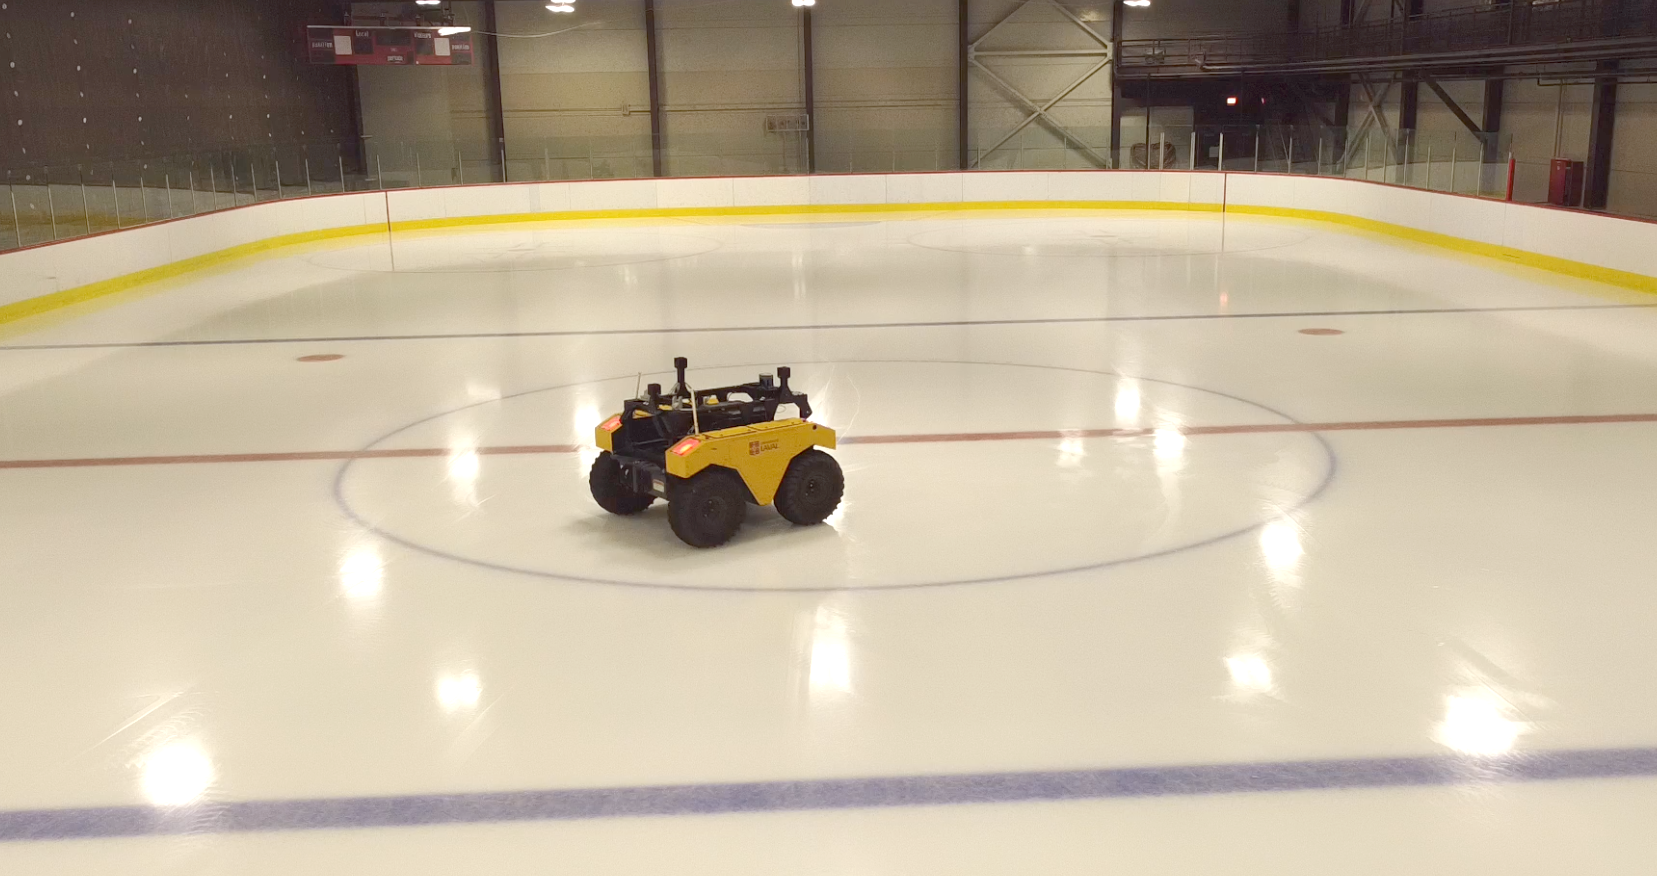
\includegraphics[width=0.7\textwidth]{figs/warthog_ice.png}
%	\caption{
%		A photo is the Warthog, our~\SI{470}{\kilo\gram} research~\ac{SSMR}.
%		Via the~\ac{DRIVE} protocol, we have collected a~\SI{20}{\min} dataset of the vehicle exectuting a large spectrum of commands.
%		This dataset shows the limit of our current slip learning model, motivating an investigation of dynamic model performance.
%	}
%	\label{fig:warthog-ice}
%\end{SCfigure}

%This work could lead to contributions related to the dynamic model formulation for~\acp{SSMR} navigating on ice, or learning dynamic model parameters through~\ac{BLR} to facilitate deployment of dynamic models.
%The evaluation pipeline for model training and prediction error over an entire dataset is already set up and ready to compare dynamic models to slip learning.\footnote{\url{https://github.com/norlab-ulaval/norlab_WMRD}}
%Improvements could also be made to the~\ac{DRIVE} protocol to sample additional dynamic variables, such as body acceleration.
%\subsection{Adaptive motion modeling}
%Next, I plan to study the performance of adaptive modeling under extreme traction variation.
%To illustrate this challenge, \autoref{fig:snow_var} shows two use cases, namely hard and deep snow navigation, for which traction varies significantly.
%In the case of deep snow navigation, the~\ac{SSMR} almost reached immobilization, which means that switching between both conditions produces the largest change in traction conditions that can be observed for a specific~\ac{UGV}.
%This is an ideal case to investigate the limits of current adaptive modeling approach, which is easy to integrate with our slip learning model.
%\begin{figure}[h!]
%	\begin{center}
%		\begin{subfigure}[b]{0.49\textwidth}
%			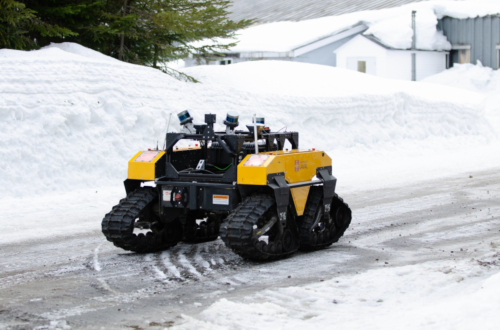
\includegraphics[width=\linewidth]{figs/warthog_hard_snow.pdf}
%			\caption{}
%			\label{fig:hard_snow}
%		\end{subfigure}%
%		~
%		\begin{subfigure}[b]{0.49\textwidth}
%			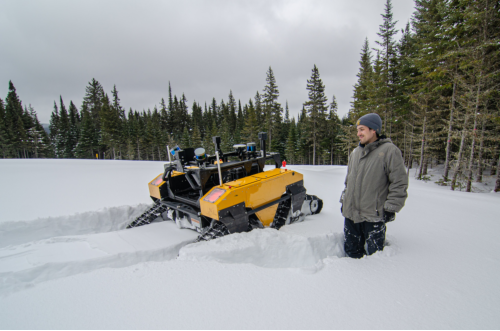
\includegraphics[width=\linewidth]{figs/snow_depth.pdf}
%			\caption{}
%			\label{fig:deep_snow}
%		\end{subfigure}%
%		\caption{
%			Example of distinct terrain navigating encountered during wintertime off-road navigation with the Warthog platform.
%			\textbf{(a)}: Hard snow navigation, with limited slip, representing nominal navigation.
%			\textbf{(b)}: Deep snow navigation, with high slip, representing an edge case for~\ac{SSMR} motion modeling.
%		}
%		\label{fig:snow_var}
%	\end{center}
%\end{figure}

%As proposed by~\citet{Mckinnon2019}, weighted~\ac{BLR} learning enables re-training of the model based on new traction conditions and a prior motion model.
%In their work, they show that weighted~\ac{BLR} performs well in adapting to slight changes in traction conditions, both artificially generated and through slope variation.
%However, no study has investigated the performance of adaptive modeling with respect to the degree of traction variability and what is the operational limit.
%By leveraging the~\ac{DRIVE} protocol to gather two distinct datasets, namely on hard and deep snow, we could simulate such changes in traction and analyse the performance of weighted~\ac{BLR} learning.
%In the case of failure, it will be an opportunity to develop improvements to this adaptive modeling approach, increasing its robustness to significant variation in traction.

%\subsection{\ac{DRIVE} impact on path following}
We have developed a predictive control library in the context of industrial demonstrations for this project.\footnote{\url{https://github.com/norlab-ulaval/norlab_controllers}}
Such controllers are based on the~\ac{MPC} algorithm, enabling high-speed path following with low tracking error.
In our case, we have implemented a simplified version of the slip-aware~\ac{MPC} controlled proposed by~\citet{Hewing2020}.
Since the motion model acts as an interchangeable module for such controllers, the prediction accuracy improvements reached through our work on the~\ac{DRIVE} protocol will most likely improve~\ac{MPC} path following performance.
A last interesting result would be to quantify the path following error improvement reached through training the slip learning model with a~\ac{DRIVE}-gathered training dataset instead of manual driving.
Typically, human driving data is limited in driving velocity since it is the first time for which the vehicle navigated the target trajectory.
Our hypothesis is that by training the model through~\ac{DRIVE}, path following performance at high speed is improved as soon as the first time the~\ac{UGV} executes the desired trajectory.

\subsection{Schedule for upcoming work}
\label{sec:schedule}

In this section, a plan for the upcoming steps for this thesis is presented. 
A Gantt chart is shown in~\autoref{fig:gantt}, providing visual support for the planning presented.
The remaining work is split into three main categories, namely thesis writing, \emph{ICRA} paper finalization and thesis review and defense.
\setlength{\fboxsep}{9pt}
\begin{figure}[h!]
	\centering
	\definecolor{navyblue}{RGB}{21,80,130}
\setganttlinklabel{f-s}{}

\begin{ganttchart}[
     %Specs 0.43 0.43 1
     y unit title=0.43cm,
     y unit chart=0.55cm,
     x unit=1.1cm,  %1.2cm
     vgrid={*{1}{draw=none},*{1}{black}},
     title height=1,   %1
     title label font=\bfseries\footnotesize,
     % bar 0.4 10pts
     bar/.style={fill=navyblue},
     bar height=0.4,
     bar label font=\footnotesize,
     bar label node/.append style={left=10pt},  %10
     % group 0 0.6 0.3 0.2 0.3 10pts
     group right shift=0,
     group top shift=0.6,
     group height=.3,
     group peaks width={0.2},
     group peaks height={0.3},
     group label node/.append style={left=10pt},
     group label font=\bfseries\footnotesize,
     % milestone 0.4 1 10pts
     milestone/.append style={xscale=0.4, yscale=1},
     milestone label node/.append style={left=10pt},
     milestone label font=\itshape\footnotesize
     ]{1}{8}
    \gantttitle[]{2024}{8}
    \\              
    \gantttitle{J}{1} \gantttitle{F}{1} \gantttitle{M}{1} 
    \gantttitle{A}{1} \gantttitle{M}{1} \gantttitle{J}{1} 
    \gantttitle{J}{1} \gantttitle{A}{1} 
    \\
    %--------------------------------------       
    \ganttgroup{Thesis writing}{1}{3}\\
    
    \ganttbar{Articles insertion}{1}{1}
    \ganttbar[inline, bar label font/.append=\color{white}]{}{1}{1}\\
    
    \ganttbar{Final results chapter}{2}{2}
    \ganttbar[inline, bar label font/.append=\color{white}]{}{2}{2}\\
    
    \ganttbar{Introduction, conclusion}{3}{3}
    \ganttbar[inline, bar label font/.append=\color{white}]{}{3}{3}\\
	
	\ganttmilestone{Thesis submitted}{3}\\
	
    %--------------------------------------       
    \ganttgroup{Final experiments}{1}{2} \\ 
    
    \ganttbar{DRIVE impact on UGV path following}{1}{2}
    \ganttbar[inline, bar label font/.append=\color{white}]{}{1}{2}\\
    
    %--------------------------------------       
    \ganttgroup{\emph{ICRA 2024}}{2}{5} \\ 
    
    \ganttbar{Paper corrections}{2}{2}
    \ganttbar[inline, bar label font/.append=\color{white}]{}{2}{2}\\
    
    \ganttmilestone{Re-submission}{2}\\
    
    \ganttbar{Presentation preparation}{5}{5}
    \ganttbar[inline, bar label font/.append=\color{white}]{}{5}{5}\\
    
    \ganttmilestone{Article presentation}{5}\\
    
    %--------------------------------------       
    \ganttgroup{Thesis defense}{4}{8}\\
    
    \ganttbar{Thesis review}{4}{6}
    \ganttbar[inline, bar label font/.append=\color{white}]{}{4}{6}\\
    
    \ganttbar{Defense preparation}{4}{6}
    \ganttbar[inline, bar label font/.append=\color{white}]{}{4}{6}\\
    
    \ganttmilestone{Defense}{6}\\
    
    \ganttbar{Final reviews}{7}{8}
    \ganttbar[inline, bar label font/.append=\color{white}]{}{7}{8}\\
    
    \ganttmilestone{Final submission}{8}\\
    
\end{ganttchart}

	\caption{Gantt chart of the remaining tasks left to complete this thesis and planning for their completion leading to August 2024.}
	\label{fig:gantt}
\end{figure}
\setlength{\fboxsep}{12pt}

The thesis will be written via article insertion, where the articles selected are presented in~\autoref{sec:first_author}.
This task will require appending every article which will represent a distinct thesis chapter.
Mathematical notation will be modified to be uniform for all articles and facilitate thesis reading and review.
Then, I will write on writing the final chapter, which will present the results of the experiments described in~\autoref{sec:future_work}.
My planning is to invest half days on thesis writing and the other half days on final experiments to maintain motivation through the writing process.
%For these final experiments, I will focus on dynamic modeling during the first two months since the data is already recorded and the result can be produced generally faster.
%Then, when winter comes, I will record the data for the hard and deep snow experiments and produce the results in the first two months of 2024.
Final chapter writing will be done after those last experiments are conducted.
%An optional extra paper will be written between the initial thesis submission and thesis defense if the final results are conclusive and time allows.
%For this work, the target publication venue will most likely be~\emph{IEEE Robotics and Automation Letters (RAL)}.\footnote{\url{https://www.ieee-ras.org/publications/ra-l}}

Furthermore, since our work on~\ac{DRIVE} is undergoing the peer review process, we will receive the results in January 2024.
Paper improvements will need to be prioritized at this time for paper re-submission which will most likely be due at the end of January 2024.
Then, the official paper presentation will be done during the three weeks leading to the conference, including a dry run in the laboratory to fetch initial feedback and maximize the presentation quality.
Then, from May 14th to 17th 2024, I will attend the conference to present our paper on-site.
In the case the paper is rejected at the conference, the reviews will still be into account and the paper will be improved and re-submitted to an alternative venue.
In this case, slight changes to the planning presented in this section will be made to ensure thesis defense still happens in August 2024.

Lastly, once the thesis is submitted, we will follow standard academic delays defined by Université Laval for review, corrections and defense.
A total of five months is scheduled between thesis submission and graduation, up to August 2024.
This will allow time to validate the initial submission, have the committee review it, defend the thesis and produce the final version.
With around a month of contingency, this planning will conclude the work done on this thesis.

\section{Conclusion}
\label{sec:conclusion}

In this document, we have described the current scientific work completed in the realization of this thesis.
In total, I have published one conference paper and one journal paper and submitted another conference paper as the first author.
Meanwhile, I have taken part in an additional four papers as a co-author.
This scientific production will represent the majority of the content of my article insertion thesis.

For the last chapter of the thesis, I have identified three last experiments which would be relatively simple to complete considering the amount of work already completed.
Providing these results are conclusive, they will be added in the final chapter of my thesis.
The initial thesis submission is scheduled for March 2024, leading to the defense in August 2024 according to Université Laval standards.


% ---------------------------------------------------------------
\printbibliography
%\newpage

% ---------------------------------------------------------------
%\begin{landscape}
%\section{Annexe}
\label{sec:Annexe}

\setlength{\fboxsep}{9pt}
\begin{figure}[htbp]
  \centering
  \definecolor{navyblue}{RGB}{21,80,130}
\setganttlinklabel{f-s}{}

\begin{ganttchart}[
     %Specs 0.43 0.43 1
     y unit title=0.43cm,
     y unit chart=0.37cm,
     x unit=0.7cm,  %1.2cm
     vgrid={*{3}{draw=none},*{1}{black}},
     title height=1,   %1
     title label font=\bfseries\footnotesize,
     % bar 0.4 10pts
     bar/.style={fill=navyblue},
     bar height=0.4,
     bar label font=\footnotesize,
     bar label node/.append style={left=10pt},  %10
     % group 0 0.6 0.3 0.2 0.3 10pts
     group right shift=0,
     group top shift=0.6,
     group height=.3,
     group peaks width={0.2},
     group peaks height={0.3},
     group label node/.append style={left=10pt},
     group label font=\bfseries\footnotesize,
     % milestone 0.4 1 10pts
     milestone/.append style={xscale=0.4, yscale=1},
     milestone label node/.append style={left=10pt},
     milestone label font=\itshape\footnotesize
     ]{1}{20}
    \gantttitle[]{2022}{8}
    \gantttitle[]{2023}{12}
    \\              
    \gantttitle{N1}{1} \gantttitle{N2}{1} \gantttitle{N3}{1} \gantttitle{N4}{1} \gantttitle{D1}{1} \gantttitle{D2}{1} \gantttitle{D3}{1} \gantttitle{D4}{1} \gantttitle{J1}{1} \gantttitle{J2}{1} \gantttitle{J3}{1} \gantttitle{J4}{1}
    \gantttitle{F1}{1} \gantttitle{F2}{1} \gantttitle{F3}{1} \gantttitle{F4}{1} \gantttitle{M1}{1} \gantttitle{M2}{1} \gantttitle{M3}{1} \gantttitle{M4}{1}
    \\
    %--------------------------------------       
    \ganttgroup{Déploiements et expériences}{1}{6}\\
    
    \ganttbar{Performances système}{1}{1}
    \ganttbar[inline, bar label font/.append=\color{white}]{}{1}{1}\\
    
    \ganttbar{Tests positions prismes}{2}{2}
    \ganttbar[inline, bar label font/.append=\color{white}]{}{2}{2}\\
    
    \ganttbar{Comparaison GNSS}{2}{5}
    \ganttbar[inline, bar label font/.append=\color{white}]{}{2}{5}\\
    
    \ganttbar{Déploiement forêt 1}{2}{2}
    \ganttbar[inline, bar label font/.append=\color{white}]{}{2}{2}\\
    
    \ganttbar{Déploiement forêt 2}{5}{5}
    \ganttbar[inline, bar label font/.append=\color{white}]{}{5}{5}\\
	
	\ganttmilestone{Ensemble des données récoltées}{6}\\
	
    %--------------------------------------       
    \ganttgroup{Reconstruction des trajectoires}{1}{8} \\ 
    
    \ganttbar{État de l'art}{1}{2}
    \ganttbar[inline, bar label font/.append=\color{white}]{}{1}{2}\\
    
    \ganttbar{Génération vérités terrains}{1}{4}
    \ganttbar[inline, bar label font/.append=\color{white}]{}{1}{4}\\
    
    \ganttbar{Tests méthodes interpolations}{1}{8}
    \ganttbar[inline, bar label font/.append=\color{white}]{}{1}{8}\\
    
    \ganttmilestone{Pipeline de génération fini}{8}\\
    
     %--------------------------------------       
    \ganttgroup{Utilisation de l'incertitude}{1}{12} \\ 
    
    \ganttbar{Impact positions des prismes}{1}{2}
    \ganttbar[inline, bar label font/.append=\color{white}]{}{1}{2}\\
    
    \ganttbar{Interpolation données brutes}{6}{8}
    \ganttbar[inline, bar label font/.append=\color{white}]{}{6}{8}\\
    
    \ganttbar{Obtention de l'incertitude}{8}{12}
    \ganttbar[inline, bar label font/.append=\color{white}]{}{8}{12}\\
    
    \ganttmilestone{Incertitude peut être évaluée}{12}\\
    
    %--------------------------------------       
    \ganttgroup{Évaluation de trajectoires}{3}{16} \\ 
    
    \ganttbar{Comparaison lidar-GNSS}{3}{5}
    \ganttbar[inline, bar label font/.append=\color{white}]{}{3}{5}\\
    
    \ganttbar{Comparaison des normes}{5}{8}
    \ganttbar[inline, bar label font/.append=\color{white}]{}{5}{8}\\
    
    \ganttbar{Usage de l'incertitude}{8}{12}
    \ganttbar[inline, bar label font/.append=\color{white}]{}{8}{12}\\
    
    \ganttbar{Niveau de précision}{12}{16}
    \ganttbar[inline, bar label font/.append=\color{white}]{}{12}{16}\\
    
    \ganttmilestone{Pipeline d'évaluation complété}{16}\\
    
    %--------------------------------------       
    \ganttgroup{Rédaction du journal}{1}{19} \\ 
    
    \ganttbar{Rédaction état de l'art}{1}{6}
    \ganttbar[inline, bar label font/.append=\color{white}]{}{1}{6}\\
    
    \ganttbar{Rédaction théorie}{3}{16}
    \ganttbar[inline, bar label font/.append=\color{white}]{}{4}{16}\\
    
    \ganttbar{Rédaction expériences}{6}{10}
    \ganttbar[inline, bar label font/.append=\color{white}]{}{6}{10}\\
    
    \ganttbar{Rédaction résultats}{10}{19}
    \ganttbar[inline, bar label font/.append=\color{white}]{}{10}{19}\\
    
    \ganttmilestone{Soumission du papier}{19}\\
    
\end{ganttchart}

  \caption{Diagramme de Gantt contenant les objectifs de recherche devant être accomplis d'ici au dépôt initial de la thèse pour la soumission de l'article de journal.
  }
  \label{fig:gantt_recherche}
\end{figure}
\setlength{\fboxsep}{12pt}
%\end{landscape}
%\newpage

\end{document}

